% Условная компиляция для самостоятельной работы
\ifdefined\mainfile
    % Если это часть основного файла, не добавляем начало и конец документа
\else
    \documentclass[12pt, a4paper]{report}
    \usepackage{/Users/vladbelousov/Desktop/Semestr_4-FP-NSU/Настройка/library}
    \usepackage[utf8]{inputenc} % Подключение поддержки UTF-8
    \begin{document}
\fi

%%-------------------------------%%

\begin{proof} \(  \) 

    1) Дано: \( \forall  \lambda_j (A ) \text{ }  Re \lambda_j (A ) < 0 \). Пусть \( C  = E \), \(  E = E^* > 0 \). Тогда по Теореме 3 \( \exists  ! H = H^* > 0  \) - решение матричного уравнения \( HA + A ^* H = - E . \) 

    Рассмотрим функцию \( V(\vec{ y} ) = ( H \vec{ y}  , \vec{ y} ) \). Покажем, что \( V(\vec{ y} ) \) - функция Ляпунова: 

    \( \kern+0.5cm  \) 1. \( V(\vec{ y} ) = (H \vec{ y}  , \vec{y }  ) \in  C ^1 (\left\lVert  \vec{ y}  \right\rVert < r ) \), где \( r  \) - любое; 

    \( \kern+0.5cm  \) 2. \( V(\vec{ 0}  ) = (H \vec{ 0}  , \vec{ 0 } ) = 0 , \text{ }  V (\vec{ y}  ) = (H \vec{ y}  , \vec{ y}  ) > 0 \) при \( \vec{ y }  \neq  \vec{0 }  \), так как \( H = H ^*>0 \) 

    \( \kern+0.5cm  \) 3. \(( \nabla V \vec{y }  , \vec{f }  (\vec{ y}  )) < 0  \) - ? 

    Пусть \( \vec{ y }  (t )  \) - решение \( \begin{cases}
    \displaystyle  \frac{d}{dt }  \vec{ y}  = \vec{f }(\vec{ y} ) = A  \vec{ y}  + \vec{g }  (\vec{ y} )  \\ 
    \vec{y }  (t_0 )= \vec{ y}  _0 \neq  \vec{ 0} 
    \end{cases} \) 

    , где \( \vec{ g } (\vec{ y} ) = o (\left\lVert \vec{y}  \right\rVert) \) 

    \[ \frac{d}{dt }  V (\vec{ y} (t )) = \frac{d}{dt }  V (y_1 (t ) ,..., y_n (t )) = \frac{\partial  V }{\partial  y_1 } (\vec{ y }  (t ) ) \underbrace{\frac{d y_1 (t )}{dt }}_{f_1 (\vec{ y}  (t))} + ...+  \frac{\partial  V }{\partial  y_n } (\vec{ y}  (t ))\underbrace{ \frac{d y_n (t )}{dt }}_{f_n (\vec{y } (t))}   = (\nabla V (\vec{ y}  (t )) , \vec{ f }  (\vec{ y }  (t)))\]  

    С другой стороны: 

    \[ \frac{d}{dt }  V (\vec{ y}  (t )) = \frac{d}{dt }  (H \vec{ y}  (t ) , \vec{ y}  (t )) = \bigg( H\underbrace{ \frac{d}{dt } \vec{ y}}_{\vec{ f   } (\vec{ y}  (t)) }  (t ), \vec{ y}  (t ) \bigg) + \bigg(  H \vec{ y}  (t ) , \underbrace{\frac{d}{dt }  \vec{ y }  (t)}_{\vec{ f } (\vec{ y}  (t))} \bigg) =\] 
    \[ = \bigg(  H (A \vec{ y}  (t ) + \vec{ g }  (\vec{ y}  (t ))) , \vec{ y}  (t ) \bigg)  + \bigg(  H \vec{ y}  (t ) , A \vec{ y}  (t ) + \vec{ g }  (\vec{ y }  (t)) \bigg)  = \] 
    \[  = (H A \vec{ y}  (t ) , \vec{ y}  (t ) ) + (H \vec{ g }  (\vec{ y }  (t ))) + (H \vec{ y } (t ) , A \vec{ y}  (t )) + ( H \vec{ y}  (t ) , \vec{ g }(\vec{ y}  (t)) ) = \] 
    \[ = \underbrace{(\underbrace{(H A + A ^* H )}_{= - E }\vec{ y}  (t ) ,\vec{ y}  (t ) )}_{(*)} + \underbrace{(H \vec{ g }  (\vec{ y } (t )), \vec{ y}  (t ))}_{\le  \left\lVert  H \vec{ g }  (\vec{ y}  (t ) ) \right\rVert \left\lVert  \vec{ y}  (t) \right\rVert}+ \underbrace{(H \vec{ y}  (t ) , \vec{ g }  (\vec{y }  (t))) }_{\le  \left\lVert  H \vec{ y}  (t ) \right\rVert \left\lVert  \vec{ g }  (\vec{ y } (t) ) \right\rVert} \boxed{\le }\]  
    , где \( (* ) = - (\vec{ y } (t ) , \vec{ y}  (t )) = - y_1 ^2 (t )  - ... - y_n ^2 (t ) = - \left\lVert \vec{y }  (t) \right\rVert _2 ^2  \). Тогда по неравенству Коши-Буняковского: 
    
    \[ \boxed{\le  } - \left\lVert  \vec{ y}   \right\rVert _2   ^2  + 2 \left\lVert H  \right\rVert _2  \left\lVert \vec{ g }  (\vec{ y}  (t ) ) \right\rVert  _2 \left\lVert \vec{ y }  (t) \right\rVert _2  =- \left\lVert  \vec{ y}  (t ) \right\rVert _2 ^2 \left( 1 - 2  \left\lVert  H  \right\rVert _2 \frac{ \left\lVert \vec{ g }  (\vec{ y }  (t)) \right\rVert _2 }{\left\lVert \vec{ y}  (t ) \right\rVert _2 }  \right) \] 
    , если \( \vec{ y}  (t ) \neq  0 \) 

    Если \( \vec{ y } _0 \neq  \vec{ 0}    \), то \( \vec{ y}  (t ) \neq  0\text{ }   \forall  t \in  (\alpha , \omega)\). 
    
    От противного: Если \( \exists  t_1 : \vec{ y}  (t_1 ) = \vec{ 0 }  \), то рассмотрим задачу Коши: \( \begin{cases}
    \displaystyle  \frac{d}{dt }  \vec{ y}  = \vec{ f } (\vec{ y}   ) \\ 
    \vec{ y}  (t_1 ) = \vec{ 0 }  
    \end{cases}  \Rightarrow \exists ! \) решение \( \vec{ y }  (t ) = 0 \) 

    Противоречие с тем, что \( \vec{ y}  (t_0) = \vec{ y  } _0 \neq  0 \) 

    Пусть \( t = t_0 : \displaystyle  \frac{d}{dt }  V (\vec{ y}  (t )) |_{t = t_0 } = \nabla V (\vec{y } _0 ) , \vec{ f }  (\vec{ y }  _0 )   \le  - \left\lVert y_0    \right\rVert _2 ^2 \left( 1 - 2 \left\lVert H  \right\rVert _2 \frac{ \left\lVert \vec{ g } (\vec{ y } _0 ) \right\rVert _2 }{\left\lVert \vec{ y}  _0  \right\rVert _2 }  \right) \) 

    Из условия (2) \( \Rightarrow \displaystyle  \lim_{\left\lVert \vec{y }  _0      \right\rVert \to 0 } \frac{\left\lVert  \vec{g }  (\vec{ y} _0 ) \right\rVert}{\left\lVert \vec{ y}  _0  \right\rVert } =0   \), то есть \( \forall  \varepsilon > 0 \text{ }  \exists  \delta> 0 \text{ }  \forall  \left\lVert \vec{ y}  _0  \right\rVert : \left\lVert \vec{ y}  _0  \right\rVert < \delta \Rightarrow \displaystyle  \frac{ \left\lVert \vec{ g }  (\vec{ y }_ 0 ) \right\rVert}{\left\lVert  \vec{ y}  _0 \right\rVert} < \varepsilon   \) 

    Возьмем \( \displaystyle  \varepsilon = \frac{1}{ 2 \left\lVert H  \right\rVert _2 } \Rightarrow \exists  \delta : \left\lVert  \vec{ y}  _0  \right\rVert < \delta \Rightarrow \frac{ \left\lVert \vec{g }  (\vec{ y }  _0 ) \right\rVert}{\left\lVert \vec{ y } _0  \right\rVert} < \varepsilon = \frac{1}{2 \left\lVert H  \right\rVert _2 } \Rightarrow    \) 
    
    \( (\nabla V (\vec{ y}  _0 ), \vec{f }  ( \vec{ y }  _0 )) < 0  , \text{ }  0 \le  \left\lVert \vec{y }_0   \right\rVert < r = \delta \) 

    По Теореме Ляпунова об асимптотической устойчивости \( \exists  V (\vec{ y}  ) \Rightarrow \vec{ y}  ^*     (t ) = 0  \)  -асимптотически устойчиво.

    2) Без доказательства.

\end{proof}

\section{Устойчивость положений равновесия } 

\[ \frac{d}{dt } \vec{ y}  = \vec{f }  (\vec{ y } ) \tag{1}  \] 
, где \( f_j \in  C^1 (\mathbb{D}) \) 

\begin{definition}
    Положение равновесия -  это решение \( \vec{ y }^* = \vec{ c }  \), \( \vec{ c }  \) - постоянный вектор \( \Rightarrow \vec{f }  (\vec{ c } ) = \vec{ 0}  \) 
\end{definition}

Замена \( \vec{ z }  (t ) = \vec{ y}  (t ) - \vec{ c }   \): 

\[ (1 ) \Rightarrow \frac{d}{dt }  \vec{z }  (t ) = \frac{d}{dt }  \vec{ y}  (t ) = \vec{f }  (\vec{ y}  (t )) = \vec{f }  (\vec{z  } (t ) + \vec{ c } ) \]  
\[ \frac{d}{dt }  \vec{ z } (t ) = \vec{ f }  (\vec{ z}  + \vec{ c }  ) \] 
, где \( \vec{ z }  ^* (t ) = 0 \) - решение. 

\[ \frac{d}{dt }  \vec{ z }  (t ) = \vec{ f } (\vec{ z}  + \vec{ c}  ) = \vec{f } (\vec{c } ) + \underbrace{\frac{\partial  \vec{ f } }{\partial  \vec{ z } }(\vec{ c } ) \vec{ z } }_{A }    + o (\left\lVert  \vec{z }  \right\rVert)  \] 
\[ A = \frac{\partial  \vec{f } }{\partial  \vec{z } } (\vec{ c } ) = \frac{\partial  \vec{ f } }{\partial  \vec{ y } } (\vec{ c }  )   \] 

\begin{theorem}[Теорема об устойчивости положений равновесия]
    Пусть \( A = \displaystyle  \frac{\partial  \vec{ f } }{\partial  \vec{ y} }(\vec{ c } )  \). Тогда: 

    1) \( \forall  \lambda_j \text{ }  Re \lambda_j (A ) < 0 \Rightarrow \vec{ y}  ^* (t ) = \vec{ c }   \) - асимптотически устойчиво; 

    2) \(  \exists  \lambda_k (A ) \text{ }  Re \lambda_k (A ) >0 \Rightarrow \vec{ y}  ^* (t ) = \vec{ c } \) - неустойчиво.
\end{theorem}

\chapter{Фазовые портреты автономных систем}

\section{Свойства фазовых  траекторий }

\[ \frac{d}{dt }  \vec{ y}  = \vec{f }  (\vec{ y }  ) \tag{1 } \] 
, где \( f_j \in  C^1 (\mathbb{D}) \) 

\begin{lemma}
    Пусть \( \vec{ y}  (t ) , \text{ }   t \in  (\alpha , \omega ) \) - непродолжаемое решение системы (1). Тогда \( \forall  c \in  \mathbb{R}      \text{ }  \vec{ y}  (t + c ) , \text{ }  t \in  (\alpha - c , \omega  - c ) \) - тоже непродолжаемое решение системы (1).
\end{lemma}
\begin{proof}
Очевидно, что очевидно.
\end{proof}

\begin{center}
    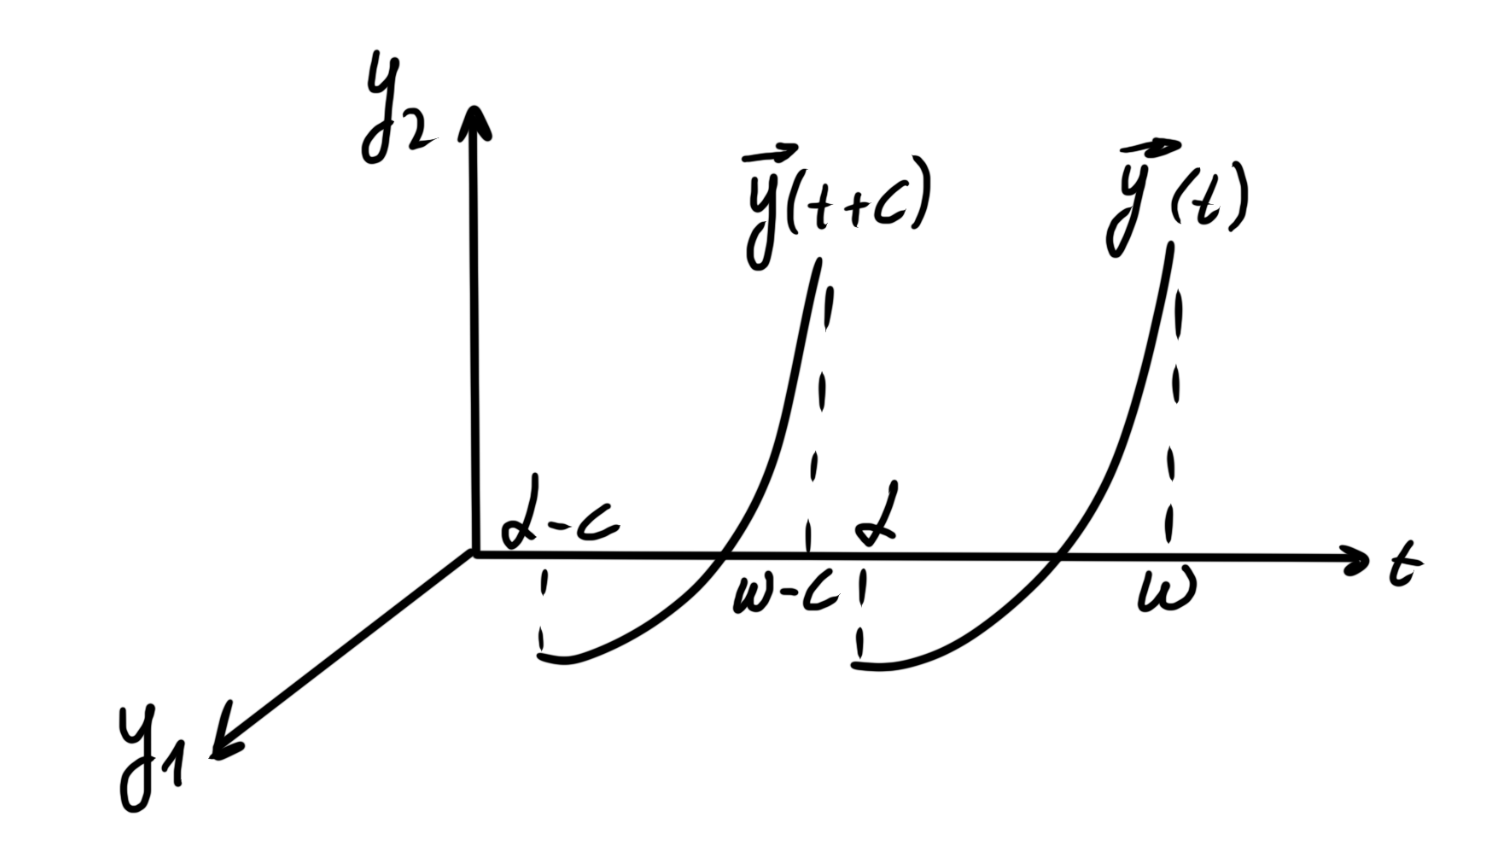
\includegraphics[width=0.6\textwidth]{/Users/vladbelousov/Desktop/Semestr_4-FP-NSU/ДфУ/Лекции_по_дням/image/64.png}
\end{center}

\begin{theorem}
    Пусть \(\begin{aligned}
        \vec{ y } _1 (t ) , \text{ }  t \in  (\alpha_1 , \omega_1 ) \\ 
        \vec{ y }  _2 (t ) ,\text{ }  t \in  (\alpha_2 , \omega_2 )
    \end{aligned}\) - два непродолжаемых решения системы (1). Пусть \( \exists  t_1 \in  (\alpha_1 , \omega_1 ) \text{ }  \exists  t_2 \in (\alpha_2 , \omega_2 ) : \vec{ y}  _1 (t_1 ) = \vec{ y } _2 (t_2 ) \). Тогда \( \exists  c \in \mathbb{R} : \vec{ y}  _2 = \vec{ y}  _1 (t +c) \), при этом \( (\alpha_2, \omega_2) = (\alpha_1 - c , \omega_1 - c )\) 
\end{theorem}

\begin{proof} \(  \) 

    Обозначим \( \vec{ y } _0 = \vec{ y } _1 (t_1 ) = \vec{ y}  _2 (t_2) \)\\ 

    Рассмотрим задачу Коши: \( \begin{cases}
    \displaystyle \frac{d}{dt }  \vec{ y}  = \vec{ f }  (\vec{ y} )\\ 
    \vec{ y}  (t_2 ) = \vec{ y}  _0
    \end{cases} \) \( \Rightarrow \vec{ y}  _2 (t )  \) - решение, \(  t \in  (\alpha_2 , \omega_2 ) \) 

    Рассмотрим функцию \( \vec{y } _1 (t+\underbrace{ t_1 - t_2 }_{c}) \), \(  t \in  (\alpha_1 - c , \omega_1 - c) \) 

    \[ \vec{ y }  _1 (t + t_1 - t_2 ) |_{t = t_2 } = \vec{y } _1 (t_1 ) = \vec{ y}  _0  \] 

    По Теореме Пикара: \( \vec{ y } _2 (t ) = \vec{ y}  _1 (t + t_1 -t_2) \) 

\end{proof}

%%-------------------------------%%

% Закрытие документа, если файл компилируется отдельно
\ifdefined\mainfile
    % Если это основной файл, не нужно заканчивать документ
\else
    \end{document}
\fi